%package list
\documentclass{article}
\usepackage[top=3cm, bottom=3cm, outer=3cm, inner=3cm]{geometry}
\usepackage{multicol}
\usepackage{graphicx}
\usepackage{url}
%\usepackage{cite}
\usepackage{hyperref}
\usepackage{array}
%\usepackage{multicol}
\newcolumntype{x}[1]{>{\centering\arraybackslash\hspace{0pt}}p{#1}}
\usepackage{natbib}
\usepackage{pdfpages}
\usepackage{multirow}
\usepackage[normalem]{ulem}
\useunder{\uline}{\ul}{}
\usepackage{svg}
\usepackage{xcolor}
\usepackage{listings}
\lstdefinestyle{ascii-tree}{
    literate={├}{|}1 {─}{--}1 {└}{+}1 
  }
\lstset{basicstyle=\ttfamily,
  showstringspaces=false,
  commentstyle=\color{red},
  keywordstyle=\color{blue}
}
%\usepackage{booktabs}
\usepackage{caption}
\usepackage{subcaption}
\usepackage{float}
\usepackage{array}

\newcolumntype{M}[1]{>{\centering\arraybackslash}m{#1}}
\newcolumntype{N}{@{}m{0pt}@{}}


%%%%%%%%%%%%%%%%%%%%%%%%%%%%%%%%%%%%%%%%%%%%%%%%%%%%%%%%%%%%%%%%%%%%%%%%%%%%
%%%%%%%%%%%%%%%%%%%%%%%%%%%%%%%%%%%%%%%%%%%%%%%%%%%%%%%%%%%%%%%%%%%%%%%%%%%%
\newcommand{\itemEmail}{gsotocco@unsa.edu.pe}
\newcommand{\itemStudent}{Gabriel Soto Ccoya}
\newcommand{\itemCourse}{Programación Web 02}
\newcommand{\itemCourseCode}{20220583}
\newcommand{\itemSemester}{III}
\newcommand{\itemUniversity}{Universidad Nacional de San Agustín de Arequipa}
\newcommand{\itemFaculty}{Facultad de Ingeniería de Producción y Servicios}
\newcommand{\itemDepartment}{Departamento Académico de Ingeniería de Sistemas e Informática}
\newcommand{\itemSchool}{Escuela Profesional de Ingeniería de Sistemas}
\newcommand{\itemAcademic}{2023 - A}
\newcommand{\itemInput}{Del 29 Mayo 2023}
\newcommand{\itemOutput}{Al 08 Junio 2023}
\newcommand{\itemPracticeNumber}{03}
\newcommand{\itemTheme}{PYTHON}
%%%%%%%%%%%%%%%%%%%%%%%%%%%%%%%%%%%%%%%%%%%%%%%%%%%%%%%%%%%%%%%%%%%%%%%%%%%%
%%%%%%%%%%%%%%%%%%%%%%%%%%%%%%%%%%%%%%%%%%%%%%%%%%%%%%%%%%%%%%%%%%%%%%%%%%%%

\usepackage[english,spanish]{babel}
\usepackage[utf8]{inputenc}
\AtBeginDocument{\selectlanguage{spanish}}
\renewcommand{\figurename}{Figura}
\renewcommand{\refname}{Referencias}
\renewcommand{\tablename}{Tabla} %esto no funciona cuando se usa babel
\AtBeginDocument{%
	\renewcommand\tablename{Tabla}
}

\usepackage{fancyhdr}
\pagestyle{fancy}
\fancyhf{}
\setlength{\headheight}{30pt}
\renewcommand{\headrulewidth}{1pt}
\renewcommand{\footrulewidth}{1pt}
\fancyhead[L]{\raisebox{-0.2\height}{
\includegraphics[width=3cm]{img/logo_episunsa.png}}}
\fancyhead[C]{\fontsize{7}{7}\selectfont	\itemUniversity \\ \itemFaculty \\ \itemDepartment \\ \itemSchool \\ \textbf{\itemCourse}}
\fancyhead[R]{\raisebox{-0.2\height}{
\includegraphics[width=1.2cm]{img/logo_abet}}}
\fancyfoot[L]{Estudiante Juan Perez Perez}
\fancyfoot[C]{\itemCourse}
\fancyfoot[R]{Página \thepage}

% para el codigo fuente
\usepackage{listings}
\usepackage{color, colortbl}
\definecolor{dkgreen}{rgb}{0,0.6,0}
\definecolor{gray}{rgb}{0.5,0.5,0.5}
\definecolor{mauve}{rgb}{0.58,0,0.82}
\definecolor{codebackground}{rgb}{0.95, 0.95, 0.92}
\definecolor{tablebackground}{rgb}{0.8, 0, 0}

\lstset{frame=tb,
	language=bash,
	aboveskip=3mm,
	belowskip=3mm,
	showstringspaces=false,
	columns=flexible,
	basicstyle={\small\ttfamily},
	numbers=none,
	numberstyle=\tiny\color{gray},
	keywordstyle=\color{blue},
	commentstyle=\color{dkgreen},
	stringstyle=\color{mauve},
	breaklines=true,
	breakatwhitespace=true,
	tabsize=3,
	backgroundcolor= \color{codebackground},
}

\begin{document}
	
	\vspace*{10px}
	
	\begin{center}	
		\fontsize{17}{17} \textbf{ Informe de Laboratorio \itemPracticeNumber}
	\end{center}
	\centerline{\textbf{\Large Tema: \itemTheme}}
	%\vspace*{0.5cm}	

	\begin{flushright}
		\begin{tabular}{|M{2.5cm}|N|}
			\hline 
			\rowcolor{tablebackground}
			\color{white} \textbf{Nota}  \\
			\hline 
			     \\[30pt]
			\hline 			
		\end{tabular}
	\end{flushright}	

	\begin{table}[H]
		\begin{tabular}{|x{4.7cm}|x{4.8cm}|x{4.8cm}|}
			\hline 
			\rowcolor{tablebackground}
			\color{white} \textbf{Estudiante} & \color{white}\textbf{Escuela}  & \color{white}\textbf{Asignatura}   \\
			\hline 
			{\itemStudent \par \itemEmail} & \itemSchool & {\itemCourse \par Semestre: \itemSemester \par Código: \itemCourseCode}     \\
			\hline 			
		\end{tabular}
	\end{table}		
	
	\begin{table}[H]
		\begin{tabular}{|x{4.7cm}|x{4.8cm}|x{4.8cm}|}
			\hline 
			\rowcolor{tablebackground}
			\color{white}\textbf{Laboratorio} & \color{white}\textbf{Tema}  & \color{white}\textbf{Duración}   \\
			\hline 
			\itemPracticeNumber & \itemTheme & 04 horas   \\
			\hline 
		\end{tabular}
	\end{table}
	
	\begin{table}[H]
		\begin{tabular}{|x{4.7cm}|x{4.8cm}|x{4.8cm}|}
			\hline 
			\rowcolor{tablebackground}
			\color{white}\textbf{Semestre académico} & \color{white}\textbf{Fecha de inicio}  & \color{white}\textbf{Fecha de entrega}   \\
			\hline 
			\itemAcademic & \itemInput &  \itemOutput  \\
			\hline 
		\end{tabular}
	\end{table}
	
	\section{Tarea}
	\begin{itemize}		
		\item Implemente los métodos de la clase Picture. Se recomienda que implemente la clase picture por etapas, probando realizar los dibujos que se muestran en la siguiente preguntas.
		\item Usando únicamente los métodos de los objetos de la clase Picture, dibuje las figuras (invocando el método "draw()").
	\end{itemize}
	
	\section{Equipos, materiales y temas utilizados}
	\begin{itemize}
		\item Sistema operativo Windows 11.
		\item Librería PyGame.
		\item Python 3.10.11.
		\item Git 2.39.2.
		\item Cuenta en GitHub con el correo institucional (GabSoto).
		\item TextMaker / GhostScript / MikTex
		\item Programación Orientada a Objetos.
		\item Manejo de matrices unidimensionales.
	\end{itemize}
	
	\section{URL de Repositorio Github}
	\begin{itemize}
		\item URL del Repositorio GitHub para clonar o recuperar.
		\item \url{https://github.com/GabSoto/Pweb02-Lab03.git}
		\item URL para el laboratorio 04 en el Repositorio GitHub.
		\item \url{https://github.com/GabSoto/Pweb02-Lab03/tree/main/Laboratorio%2003}
	\end{itemize}
	
	\section{Implementación de los métodos}
	
	\subsection{Método \textit{horizontalMirror()}}

El presente método nos pedía invertir una pieza del tablero 180°, para lograr esto se recorre el array desde atrás mientras que se va guardando estos elementos en un nuevo array.
	
		\lstinputlisting[language=Python, caption={horizontalMirror.py},numbers=left,]{src/horizontalMirror.py}
		
	\subsection{Método \textit{negative()}}

El siguiente método nos pedía invertir el color de cualquier pieza, esto usando el método ya proporcionado \_invColor(). Luego se reemplaza cada fila de los arrays por su contracolor.
	
		\lstinputlisting[language=Python, caption={negative.py},numbers=left,]{src/negative.py}

	\subsection{Método \textit{join()}}

La función de este método era poder fusionar dos imágenes en una, colocando en la derecha la imagen recibida (p). Para lograr esto,  se convirtió las imágenes en arrays con el .img para luego agregar ambos en un array new\_img.
	
		\lstinputlisting[language=Python, caption={join.py},numbers=left,]{src/join.py}
		
	\subsection{Método \textit{up()}}

Este método nos pedía guardar una imagen sobre otra, esto se logró usando el método .append, dónde agregamos el array de la imagen al final.
	
		\lstinputlisting[language=Python, caption={up.py},numbers=left,]{src/up.py}

	\subsection{Método \textit{under()}}

Esta función era para poner una imagen sobre otra, en este caso se reemplaza todos los Strings vacíos con el array de la imagen del parámetro.
	
		\lstinputlisting[language=Python, caption={under.py},numbers=left,]{src/under.py}
		
	\subsection{Método \textit{horizontalRepeat()}}

Este método constaba en imprimir (n) veces el mismo elemento de forma horizontal, funciona usado un bucle en base a (n) y el método join().
	
		\lstinputlisting[language=Python, caption={horizontalRepeat.py},numbers=left,]{src/horizontalRepeat.py}
		
	\subsection{Método \textit{verticalRepeat()}}

Este método constaba en imprimir (n) veces el mismo elemento de forma vertical, funciona usado un bucle en base a (n) y el método up().

		\lstinputlisting[language=Python, caption={verticalRepeat.py},numbers=left,]{src/verticalRepeat.py}
		
	\clearpage
	
	\section{Ejecuciones}
	
	\subsection{Ejercicio A:}
	
	\begin{figure}[H]
		\centering
		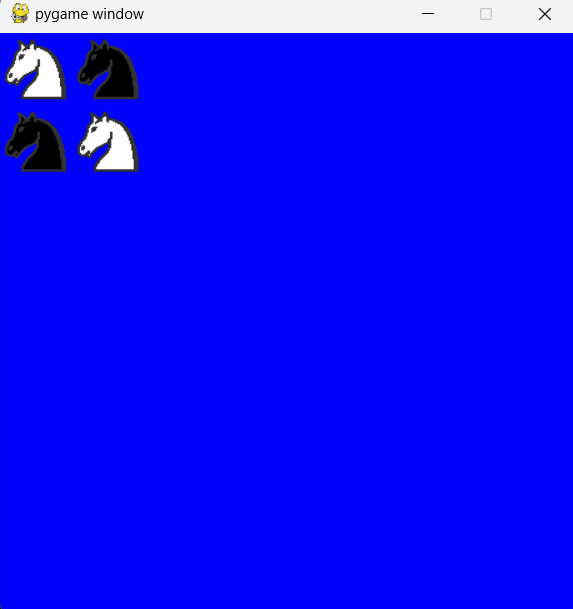
\includegraphics[width=0.55\textwidth,keepaspectratio]{img/Picture A.png}
		%\includesvg{img/automata.svg}
		%\label{img:mot2}
		%\caption{Product backlog.}
	\end{figure}	
	
	\subsection{Ejercicio B:}
	
	\begin{figure}[H]
		\centering
		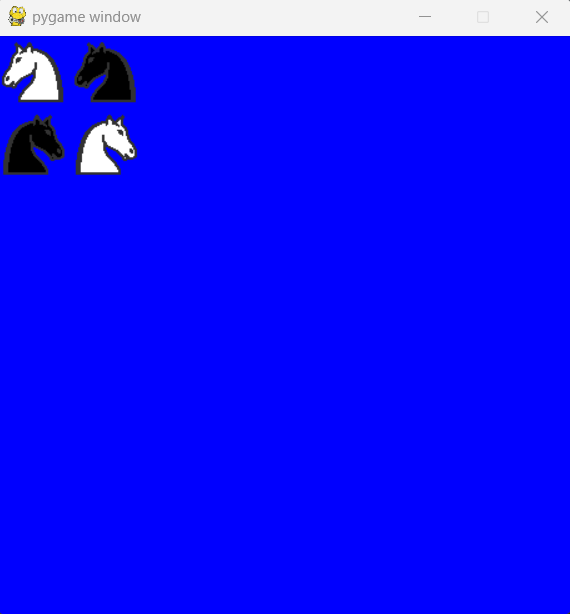
\includegraphics[width=0.55\textwidth,keepaspectratio]{img/Picture B.png}
		%\includesvg{img/automata.svg}
		%\label{img:mot2}
		%\caption{Product backlog.}
	\end{figure}	
	
	\subsection{Ejercicio C:}
	
	\begin{figure}[H]
		\centering
		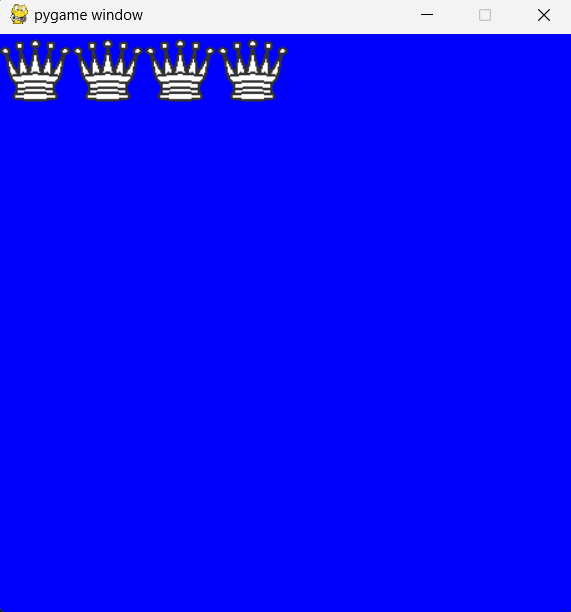
\includegraphics[width=0.55\textwidth,keepaspectratio]{img/Picture C.png}
		%\includesvg{img/automata.svg}
		%\label{img:mot2}
		%\caption{Product backlog.}
	\end{figure}	
	
	\subsection{Ejercicio D:}
	
	\begin{figure}[H]
		\centering
		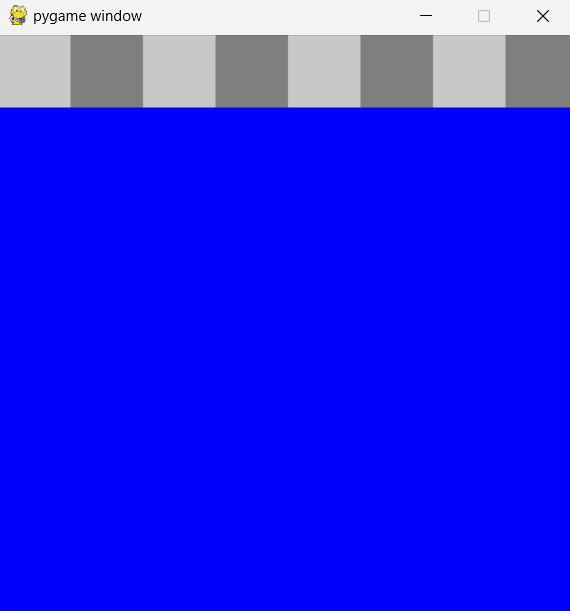
\includegraphics[width=0.55\textwidth,keepaspectratio]{img/Picture D.png}
		%\includesvg{img/automata.svg}
		%\label{img:mot2}
		%\caption{Product backlog.}
	\end{figure}	
	
	\subsection{Ejercicio E:}
	
	\begin{figure}[H]
		\centering
		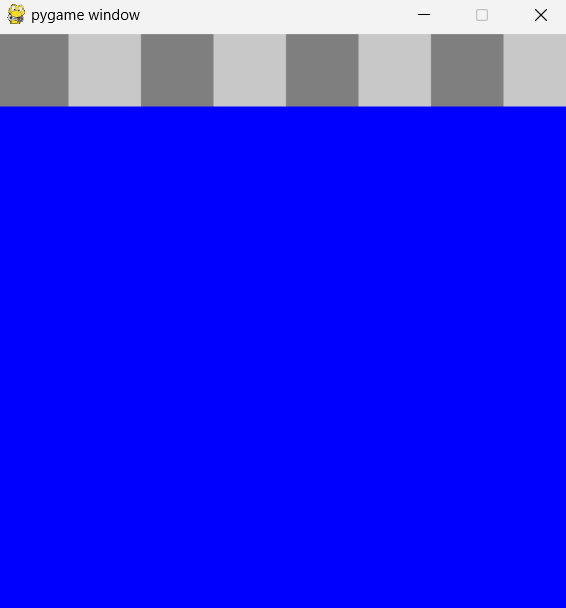
\includegraphics[width=0.55\textwidth,keepaspectratio]{img/Picture E.png}
		%\includesvg{img/automata.svg}
		%\label{img:mot2}
		%\caption{Product backlog.}
	\end{figure}	
	
	\subsection{Ejercicio F:}
	
	\begin{figure}[H]
		\centering
		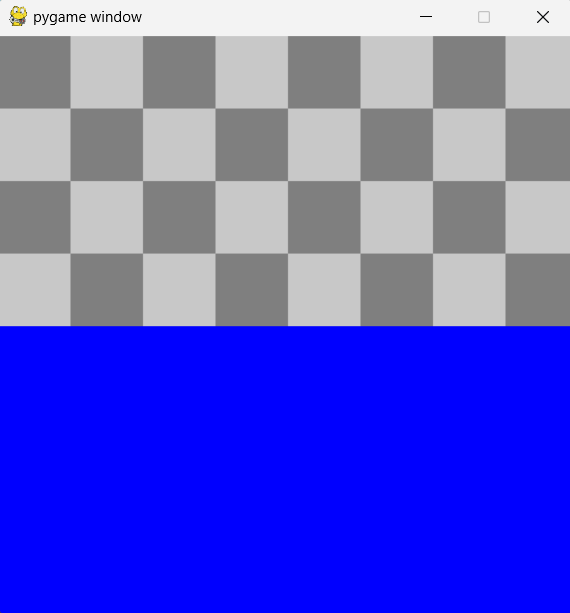
\includegraphics[width=0.55\textwidth,keepaspectratio]{img/Picture F.png}
		%\includesvg{img/automata.svg}
		%\label{img:mot2}
		%\caption{Product backlog.}
	\end{figure}	

	\subsection{Ejercicio G:}
	
	\begin{figure}[H]
		\centering
		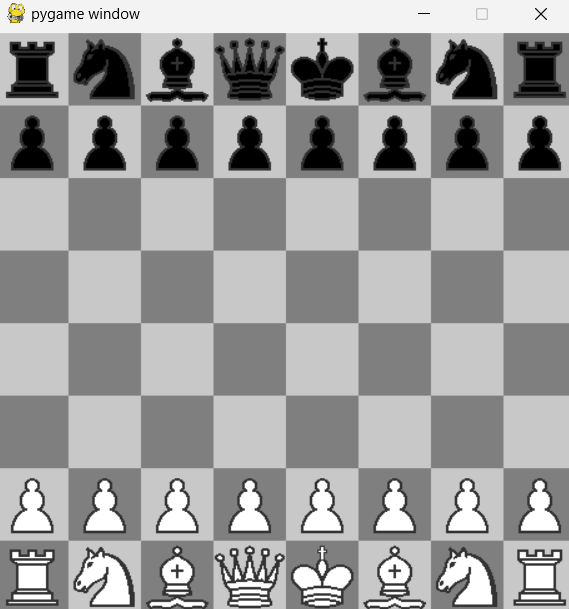
\includegraphics[width=0.55\textwidth,keepaspectratio]{img/Picture G.png}
		%\includesvg{img/automata.svg}
		%\label{img:mot2}
		%\caption{Product backlog.}
	\end{figure}	

	\subsection{Usando el método \textit{horizontalMirror()}}
	
	\begin{figure}[H]
		\centering
		
\includegraphics[width=0.55\textwidth,keepaspectratio]{img/Picture H.png}
		%\includesvg{img/automata.svg}
		%\label{img:mot2}
		%\caption{Product backlog.}
	\end{figure}		
	
		
	\subsection{Estructura de laboratorio 03}
	\begin{itemize}	
		\item El contenido que se entrega en este laboratorio es el siguiente:
	\end{itemize}
	
\begin{lstlisting}[style=ascii-tree]
Pweb2-Lab03/
|-- Laboratorio 04
|   |-- chessPictures.py
|   |-- colors.py
|   |-- Ejercicio2a.py
|   |-- Ejercicio2b.py
|   |-- Ejercicio2c.py
|   |-- Ejercicio2d.py
|   |-- Ejercicio2e.py
|   |-- Ejercicio2f.py
|   |-- Ejercicio2g.py
|   |-- interpreter.py
|   |-- picture.py
|   |-- pieces.py
|   |-- prac.py
|   |
|   |-- __pycache__
|       |-- chessPictures.cpython-310.pyc
|       |-- colors.cpython-310.pyc
|       |-- interpreter.cpython-310.pyc
|       |-- picture.cpython-310.pyc
|       |-- pieces.cpython-310.pyc
|
|-- Latex
|   |-- Laboratorio_04.aux
|   |-- Laboratorio_04.log
|   |-- Laboratorio_04.out
|   |-- Laboratorio_04.pdf
|   |-- Laboratorio_04.synctex.gz
|   |-- Laboratorio_04.tex
|   |
|   |-- img
|   |   |-- logo_abet.png
|   |   |-- logo_episunsa.png
|   |   |-- logo_unsa.jpg
|   |   |-- Picture A.png
|   |   |-- Picture B.png
|   |   |-- Picture C.png
|   |   |-- Picture D.png
|   |   |-- Picture E.png
|   |   |-- Picture F.png
|   |   |-- Picture G.png
|   |   |-- Picture H.png
|   |
|   |-- src
|       |-- horizontalMirror.py
|       |-- horizontalRepeat.py
|       |-- join.py
|       |-- negative.py
|       |-- under.py
|       |-- up.py
|       |-- verticalRepeat.py
\end{lstlisting}    

\subsection{Commits de laboratorio 03}
	
\begin{lstlisting}[language=bash,caption={Commits}][H]
commit 87a022325ef113ff075fd0092fc1e47be42348f6 (HEAD -> main, origin/main)
Author: GabSoto <gsotocco@unsa.edu.pe>
Date:   Tue Jun 6 22:06:44 2023 -0500

    Update DISPLAY and Ejercicio2g.py

commit 0a466385d51032ee2a1ebe4c823fad2af30ae50c
Author: GabSoto <gsotocco@unsa.edu.pe>
Date:   Tue Jun 6 14:47:32 2023 -0500

    Terminando el ejercicio g e implementando metodo under()

commit 2ef3d41f10eaebd145ae2d9b76129ceb7e2174b9
Author: GabSoto <gsotocco@unsa.edu.pe>
Date:   Tue Jun 6 12:54:11 2023 -0500

    Termiando el metodo horizontalMirror() e implementando un ejercicio mas para mostrar su funcionalidad.

commit 21d0a3319ffa12b82ed50981d7fc4417d48655d6
Author: GabSoto <gsotocco@unsa.edu.pe>
Date:   Tue Jun 6 12:28:27 2023 -0500

    Terminando el ejercicio f e imlementando el metodo verticalRepeat()

commit f16732866a68383cbfded968b415e5bc007669b8
Author: GabSoto <gsotocco@unsa.edu.pe>
Date:   Tue Jun 6 12:25:37 2023 -0500

    Reutilizamos el mismo metodo horizontalRepeat para este ejercicio.

commit ebfe1dabf5e9ce2db15067b4efaf2b0c9c277dd9
Author: GabSoto <gsotocco@unsa.edu.pe>
Date:   Tue Jun 6 12:24:13 2023 -0500

    Implementando el metodo horizontalRepeat() y terminando el Ejercicio d

commit 8bb3088a660b7a0c5b48a16c7159e248ddbd0a61
Author: GabSoto <gsotocco@unsa.edu.pe>
Date:   Tue Jun 6 12:22:55 2023 -0500

    corrigien el metodo up por el metodo under

commit 82b84503508477969bc6eaac74791fe7e9237c61
Author: GabSoto <gsotocco@unsa.edu.pe>
Date:   Tue Jun 6 11:39:05 2023 -0500

    Terminando el ejercicio c  e implementando el metodo horizontalRepeat()

commit ae9db59ea28960ed8e16f42c24f469174efab599
Author: GabSoto <gsotocco@unsa.edu.pe>
Date:   Tue Jun 6 10:42:18 2023 -0500

    Elaboracion del ejercicio b

commit 65e1c2b6fc485fae77fa36e495bb0e56d0c0f1eb
Author: GabSoto <gsotocco@unsa.edu.pe>
Date:   Tue Jun 6 07:41:25 2023 -0500

    Termimando el ejercicio a e implementando los metodos under() y join()

commit 7239b1d2ee08c160d4d969273fa63977da7140d8
Author: GabSoto <gsotocco@unsa.edu.pe>
Date:   Mon Jun 5 21:35:16 2023 -0500

    Implementando los metodos join() y under()

commit 1e7b36822133423c4ba833bf75f83ad9ac7ae0c0
Author: GabSoto <gsotocco@unsa.edu.pe>
Date:   Mon Jun 5 20:44:16 2023 -0500

    Implementando la funcion negative()
(END)
\end{lstlisting}

\section{Preguntas:}

	\textbf{¿Qué son los archivos *.pyc?}
	
\vspace{0.3cm}
Los archivos con extensión '.pyc' en Python son generados por el intérprete de Python como una forma de almacenar el bytecode compilado del código fuente. Cuando un archivo de Python se ejecuta por primera vez, el intérprete compila el código fuente a bytecode y guarda ese bytecode en un archivo ".pyc". Así evitando la necesidad de compilar el código nuevamente.
De manera similar, en Java, los archivos ".class" contienen el bytecode compilado a partir de los archivos de código fuente ".java". Estos archivos ".class" se utilizan para ejecutar el programa de manera eficiente sin tener que recompilar el código fuente en cada ejecución.
\vspace{0.3cm}

	\textbf{¿Para qué sirve el directorio pycache?}
	
	\vspace{0.3cm}
Aquí se almacenan los archivos compilados de los módulos: chessPictures.py, colors.py, interpreter.py, picture.py y pieces.py. Estos archivos compilados, que se encuentran en el directorio "pycache", permiten evitar la necesidad de recompilarlos cada vez que se ejecuten otros archivos que los importen.
	\vspace{0.3cm}
	
	\textbf{¿Cuáles son los usos y lo que representa el subguión en Python?}
	
	\vspace{0.3cm}
El subguión (\_) en Python tiene varios usos y significados adicionales además de ser utilizado en constructores y para indicar métodos privados de una clase (como en la clase Picture). Algunos de estos usos incluyen:
	
	\begin{itemize}
		\item \textbf{Traducción de cadenas:} En la función str.maketrans() o en el método str.translate(), puedes utilizar el subguión para indicar que un carácter debe ser eliminado o dejado sin cambios durante una operación de traducción de cadenas.
	\end{itemize}
	
	\begin{lstlisting}[language=bash,caption={Ejemplo}][H]
		translation_table = str.maketrans("aeiou","_____")
		resultado = "Hola, mundo!".translate(translation_table)
		print(resultado)			
			
		Ouput >>  H_l_, m_nd_!
	\end{lstlisting}		
	
	\begin{itemize}
		\item \textbf{Ignorar valores en desempaquetado:} Al desempaquetar una secuencia o iterador, puedes utilizar el subguión para ignorar los valores que no necesitas. 
	\end{itemize}
	
	\begin{lstlisting}[language=bash,caption={Ejemplo}][H]
		a, _, c = (1, 2, 3)
	\end{lstlisting}	
	
\vspace{0.3cm}


	\section{\textcolor{red}{Rúbricas}}
	
	\subsection{\textcolor{red}{Entregable Informe}}
	\begin{table}[H]
		\caption{Tipo de Informe}
		\setlength{\tabcolsep}{0.5em} % for the horizontal padding
		{\renewcommand{\arraystretch}{1.5}% for the vertical padding
		\begin{tabular}{|p{3cm}|p{12cm}|}
			\hline
			\multicolumn{2}{|c|}{\textbf{\textcolor{red}{Informe}}}  \\
			\hline 
			\textbf{\textcolor{red}{Latex}} & \textcolor{blue}{El informe está en formato PDF desde Latex,  con un formato limpio (buena presentación) y facil de leer.}   \\ 
			\hline 
			
			
		\end{tabular}
	}
	\end{table}
	
	\clearpage
	
	\subsection{\textcolor{red}{Rúbrica para el contenido del Informe y demostración}}
	\begin{itemize}			
		\item El alumno debe marcar o dejar en blanco en celdas de la columna \textbf{Checklist} si cumplio con el ítem correspondiente.
		\item Si un alumno supera la fecha de entrega,  su calificación será sobre la nota mínima aprobada, siempre y cuando cumpla con todos lo items.
		\item El alumno debe autocalificarse en la columna \textbf{Estudiante} de acuerdo a la siguiente tabla:
	
		\begin{table}[ht]
			\caption{Niveles de desempeño}
			\begin{center}
			\begin{tabular}{ccccc}
    			\hline
    			 & \multicolumn{4}{c}{Nivel}\\
    			\cline{1-5}
    			\textbf{Puntos} & Insatisfactorio 25\%& En Proceso 50\% & Satisfactorio 75\% & Sobresaliente 100\%\\
    			\textbf{2.0}&0.5&1.0&1.5&2.0\\
    			\textbf{4.0}&1.0&2.0&3.0&4.0\\
    		\hline
			\end{tabular}
		\end{center}
	\end{table}	
	
	\end{itemize}
	
	\begin{table}[H]
		\caption{Rúbrica para contenido del Informe y demostración}
		\setlength{\tabcolsep}{0.5em} % for the horizontal padding
		{\renewcommand{\arraystretch}{1.5}% for the vertical padding
		%\begin{center}
		\begin{tabular}{|p{2.7cm}|p{7cm}|x{1.3cm}|p{1.2cm}|p{1.5cm}|p{1.1cm}|}
			\hline
    		\multicolumn{2}{|c|}{Contenido y demostración} & Puntos & Checklist & Estudiante & Profesor\\
			\hline
			\textbf{1. GitHub} & Hay enlace URL activo del directorio para el  laboratorio hacia su repositorio GitHub con código fuente terminado y fácil de revisar. &2 &X &2 & \\ 
			\hline
			\textbf{2. Commits} &  Hay capturas de pantalla de los commits más importantes con sus explicaciones detalladas. (El profesor puede preguntar para refrendar calificación). &4 &X &3 & \\ 
			\hline 
			\textbf{3. Código fuente} &  Hay porciones de código fuente importantes con numeración y explicaciones detalladas de sus funciones. &2 &X &2 & \\ 
			\hline 
			\textbf{4. Ejecución} & Se incluyen ejecuciones/pruebas del código fuente  explicadas gradualmente. &2 &X &2 & \\ 
			\hline			
			\textbf{5. Pregunta} & Se responde con completitud a la pregunta formulada en la tarea.  (El profesor puede preguntar para refrendar calificación).  &2 &X &2 & \\ 
			\hline	
			\textbf{6. Fechas} & Las fechas de modificación del código fuente estan dentro de los plazos de fecha de entrega establecidos. &2 &X &2 & \\ 
			\hline 
			\textbf{7. Ortografía} & El documento no muestra errores ortográficos. &2 &X &2 & \\ 
			\hline 
			\textbf{8. Madurez} & El Informe muestra de manera general una evolución de la madurez del código fuente,  explicaciones puntuales pero precisas y un acabado impecable.   (El profesor puede preguntar para refrendar calificación).  &4 &X &4 & \\ 
			\hline
			\multicolumn{2}{|c|}{\textbf{Total}} &20 & &19 & \\ 
			\hline
		\end{tabular}
		%\end{center}
		%\label{tab:multicol}
		}
	\end{table}
	
\clearpage

\section{Referencias}
\begin{itemize}			
	\item Instalación de Pygame. \url{https://www.youtube.com/watch?v=RRir1Ok0pfI}
	\item Instalación de Latex. \url{https://www.youtube.com/watch?v=GNp5IuWSZA0&t=25s}
		\item Introducción a Python. \url{https://www.w3schools.com/python/python_reference.asp}
\end{itemize}
	
%\clearpage
%\bibliographystyle{apalike}
%\bibliographystyle{IEEEtranN}
%\bibliography{bibliography}
			
\end{document}